\documentclass[12pt,a4paper]{article}
\usepackage[spanish]{babel}
\usepackage[utf8]{inputenc}
\usepackage{graphicx}
\usepackage{blindtext}
\usepackage{amsmath}
\usepackage{amssymb,amsfonts,latexsym}

\begin{document}
\begin{center}
{\bfseries\Large FACULTAD DE INGENIER\'IA CIVIL SEDE SANTANDER DE QUILICHAO \par}
\vspace{1cm}
{\scshape\Large SOLUCI\'ON DE ECUACIONES DIFERENCIALES LINEALES MEDIANTE SERIES \par}
{\scshape\Large\textbf{Ecuaci\'on de Bessel}\par}
\vspace{1cm}
\begin{figure}[h!]
\centering

\includegraphics[width=8cm]{1.png} 
\end{figure}
\vspace{1cm}
{\scshape\Large \textbf{PRESENTADO POR:} \par}
{\scshape\Large Victoria Eugenia Guerrero\par}
{\scshape\Large \textbf{PRESENTADO A:} \par}
{\scshape\Large Jhonatan Collazos \par}
\vspace{1,5cm}
{\scshape\Large \textbf{UNIVERSIDAD DEL CAUCA} \par}
{\scshape\Large \textbf{ECUACIONES DIFERENCIALES} \par}
{\scshape\Large \textbf{2022} \par}
\end{center}

\tableofcontents 

\vspace{15cm}	

\section{INGENIER\'IA CIVIL}
\vspace{0,5cm}

\includegraphics[width=13cm, height=7cm]{../../Pictures/im (2).jpg}

\vspace{0,5cm}

La ingeniería civil es la disciplina de la ingeniería que emplea conocimientos de cálculo, mecánica, hidráulica y física para encargarse del diseño, construcción y mantenimiento de las infraestructuras emplazadas en el entorno, incluyendo carreteras, ferrocarriles, puentes, canales, presas, puertos, aeropuertos, diques y otras construcciones relacionadas.La ingeniería civil es la más antigua después de la ingeniería militar de ahí su nombre para distinguir las actividades civiles con las militares.

\vspace{0,5cm}
\section{ECUACI\'ON DIFERENCIAL}

\vspace{0,1cm}
Una ecuación diferencial es una ecuación matemática que relaciona una función con sus derivadas. En las matemáticas aplicadas, las funciones usualmente representan cantidades físicas, las derivadas representan sus razones de cambio y la ecuación define la relación entre ellas. Como estas relaciones son muy comunes, las ecuaciones diferenciales juegan un rol primordial en diversas disciplinas, incluyendo la ingeniería, la física, la química, la economía y la biología.

\vspace{0,1cm}
\section{SOLUCI\'ON DE ECUACIONES DIFERENCIALES LINEALES MEDIANTE SERIES}
\vspace{0,1cm}
\subsection{Ecuaci\'on de Bessel}
\text{En esta sección nos ocuparemos del estudio de la ecuación diferencial ordinaria}
 
 $$ x^{2}u^{"}(x)+ xu{'}(x)+(x^{2}-v^{2})u(x)=0 $$
 
 \textbf{con $v\geq O$, que se denomina ecuación de Bessel de orden $v$. Se trata de una ecuación diferencial ordinaria de orden dos con coeficientes no contantes. Nótese en primer lugar que la ecuación dada en (1) se reduce a la ecuación  con el cambio             
$R(r)=u(x), x =ru $ Para resolver la ecuación (2) se propone una solución que se pueda escribir en la forma}
\begin{equation*}
u(x)=\sum _{k=0}^{\infty}a_kx^{k+b}\hspace*{1cm}   (a_0\neq 0 )
\end{equation*}

\vspace{0,1cm}

  donde el exponente $b$ y los coeficientes $ak$ han de ser calculados. Sustituyendo (3) en (2) y
tras hacer algunos cálculos se llega a que la función
\begin{equation*}
J_v(x)=\sum _{k=0}^{\infty}\frac{(-1)^k}{k!T(k+v+1)}
\times\left(\frac {x}{2} \right)^{2k+v}
\end{equation*} 

\textbf{que se denomina función de Bessel de primera especie de orden $v$,es solución de la ecuación (2) Si $v \in/ N $, entonces las funciones $J_v$ y $J_{-v}$ son linealmente independientes y forman una base
del espacio de soluciones de (2), es decir, que la solución general de la ecuación de Bessel (2) es combinación lineal de $J_v$ y $J_{-v}$ Si $v\in N$ ,entonces las funciones $J_v$ y $J_{-v}$ son linealmente dependientes. De hecho, se verifica
que $J_{-v}=(-1)^{v}J_v$.Para resolver este problema se introduce la función de Bessel de segunda especie $Y_v$, la cual se define como:}
\begin{equation*}
Y_v(x)=\frac{\cos(v\pi)J_v(x)-J_{-v}(x)}{\sin(v\pi)}\hspace*{1cm}  (v\nexists N)
\end{equation*}
y finalmente

\vspace{0,1cm}
\begin{equation*}
Y_n(x)=\lim_{v \to n}Y_n(x) \hspace*{1cm} (n \in N)
\end{equation*}

\vspace{2cm}
Las funciones $J_n$ e $Y_n$ son linealmente independientes y por tanto, la solución general de (2), en el caso $v = n \in N$, es combinación lineal de $J_n$ e $Y_n$.

\section{EJERCICIO PROGRAMADO EN MATLAB}
\subsection{Función de Bessel}
La ecuación diferencial de segundo orden
\vspace{0,2cm}
\begin{equation*}
x^2\frac{d^2y}{dx^2}+x\frac{dy}{dx}+(x^2-n^2)y=0
\end{equation*}
\vspace{0,4cm}
se conoce como ecuación de Bessel. La solución de esta ecuación diferencial se escribe \vspace{0,2cm}
$$y=AJ_n(x)+BY_n(x)$$ \vspace{0,2cm} donde $A$ y $B$ son constantes que se determinan a partir de las condiciones iniciales. El índice n es un número real, aunque en los libros se proporcionan tablas de las funciones 
\vspace{0,2cm}
$J_n(x)$ y $Y_n(x)$ para valores enteros $n=0,1,2,3....$
\vspace{0,2cm}
\begin{equation*}
J_(x)=\sum _{k=0}^{\infty}\frac{(-1)^k(x/2)^{n+2k}}{k!(n+k)!}
\end{equation*}
\vspace{0,2cm}
\begin{equation*}
Y_n(x)=\frac{J_n(x)\cos(nx)-J_{-n}(x)}{\sin(nx)}
\end{equation*}

\vspace{0,6cm}
Para $n$ entero se cumple
\vspace{0,6cm}
$$J_{-n}(x)=(-1)^nJ_n(x)$$
$$Y_{-n}(x)=(-1)^n Y_n(x)$$

\vspace{3cm}
\subsection{Funciones de Bessel de primera especie}
Representamos $J_0(x)$, $J_1(x)$, $J_2(x)$ y $J_3(x)$ llamando a la función bessel $j(n,x)$ de MATLAB, dando valores a su primer parámetro $n=0,1,2,3,$

\vspace{0,6cm}
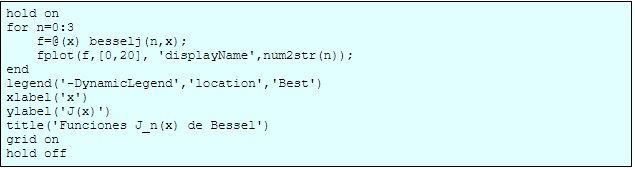
\includegraphics[width=14cm, height=6cm]{cap1.jpg} 

\vspace{0,6cm}
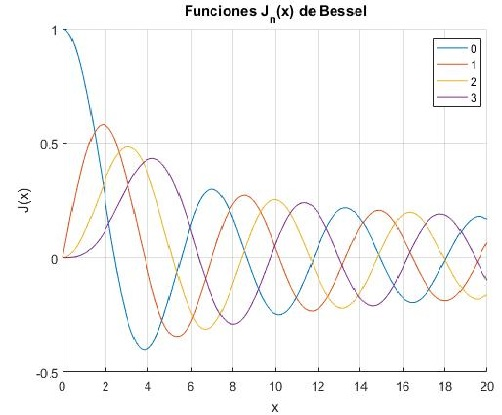
\includegraphics[width=14cm]{cap2.jpg} 
\subsection{Aproximaciones}
Cuando $x$ se hace grande la función $J_n(x)$, tiende hacia

\vspace{0,6cm}
\begin{equation*}
J_0(x)\approxeq \sqrt{\frac{2}{\pi x}}\cos (x- \frac{\pi}{4})
\end{equation*}

\begin{equation*}
J_n(x)\approxeq \sqrt{\frac{2}{\pi x}}\cos (x- \frac{n\pi}{2}-\frac{\pi}{4})
\end{equation*}

\vspace{0,6cm}
Representamos la función $J_n(x)$ y su aproximación asintótica

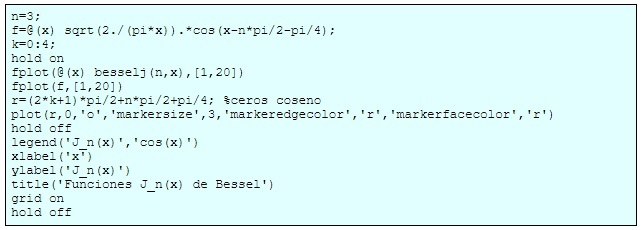
\includegraphics[width=14cm, height=10cm]{../../Pictures/Screenshots/cap 3.jpg} 

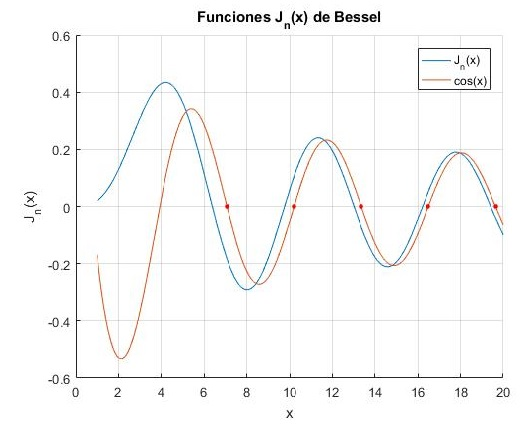
\includegraphics[width=14cm, height=12cm]{../../Pictures/Screenshots/cap4.jpg} 

\vspace{0,6cm}
En la figura, se ha representado los ceros de la función cos$(x-n\pi/2-\pi/4)$, que como vemos son próximos a los ceros de la función $J_n(x)$. Este hecho nos permite calcular los ceros de la función de Bessel mediante el comando fzero de MATLAB. Recuérdese que los ceros de la función coseno son $(2k+\pi)/2$, $k=0,1,2,3...$


\vspace{4cm}
\begin{thebibliography}{10}
\bibitem{vick}https://es.wikipedia.org/wiki/Ingenier%C3%ADa_civil 
\bibitem{vick1}https://manualdelatex.com/tutoriales/figuras 
\bibitem{vick2}https://manualdelatex.com/tutoriales/ecuaciones 
\bibitem{vick3}https://www.youtube.com/watch?v=bvKc9Z9DXPc 
\bibitem{vick0}https://www.youtube.com/watch?
\bibitem{vick5}https://www.dmae.upct.es/~fperiago/apuntesdocencia/tema7.pdf 
\end{thebibliography}
\end{document}


